\section{PVSLM}
\label{sec:pvslm}

This section describes the design and architecture of PVS Library Manager.

Before to describe and analyze the tool, is necessary to define the structure used. The smallest part are the theories, which are organized in packages. Those packages are the main element for the tool. Finally there are sets of packages, called libraries. Furthermore, it is necessary to specify the connections or relations within a library, these are the dependencies between its packages. So every package must have a dependencies list defined as the union of the dependencies of its theories.

PVSLM has been developed to manage the installation and update of packages from a PVS library. It has been divided into two sections, the first one manage the source and repository for each library, and the second one manage the packages.

The source section is divided into two parts: the configuration file and the repository. The configuration file contains the information about the library as the name, description and the URL for the git repository where it can be download. It is important to recall that the library must be available on a git server as GitHub or BitBucket. The repository is a clone of a git, that can be updated or deleted. This section is completely dedicated to the configuration of the libraries.

The other section manage the packages, their uninstall, update, list and installation, based on the already configured libraries. PVSLM is based on the dependencies graph of the library, therefore all the modifications on a package will affect the adjacent ones.

As the tool has been developed for the PVS NASA library (nasalib), this one is configured by default. All the commands available on PVSLM are listed along with their description on table \ref{tab:comm}.

\begin{table}[h!]
  \begin{center}
    \begin{tabular}{ | l | l | l | p{5cm} | }
      \hline Section & Command & Parameters & Description \\ \hline
      src & -a          & name description URL  & Create a new .list file with the library information.                   \\ \cline{2-4}
          & -d          & name                  & Delete the library .list file.                                          \\ \cline{2-4}
          & -c          & name                  & Create the library repository based on the source with the same name. 
                                                  The creation is a clone of the git repository.                          \\ \cline{2-4}
          & -u          & name                  & Update the library using a pull command.                                \\ \cline{2-4}
          & -r          & name                  & Remove the repository.                                                  \\ \hline
      pkg & -i          & library@package       & Install and update the package and all its dependencies.                \\ \cline{2-4}
          & -u          & library@package       & Update an installed package and all its dependencies.                   \\ \cline{2-4}
          & -d          & library@package       & Delete an installed package with all ones that depends on it.           \\ \cline{2-4}
          & -l          &                       & List all the installed libraries.                                       \\ \cline{2-4}
          & -l          & library               & List all the available packages of the library.                         \\ \cline{2-4}
          & -l          & library@package       & List all the dependencies of the package.                               \\ \hline
    \end{tabular}
  \end{center}
  \caption{PVS Library Manager command list}
  \label{tab:comm}
\end{table}

PVSLM works locally, but it needs Internet connection for its installation and the communication with the git repositories. Basically it is downloaded and then configured, once it is installed there are several commands that needs to connect to the git repository either to clone or pull it. For example, when a package is going to be installed, it is updated along with all its dependencies. The figure \ref{fig:archi} shows how the tool works.

\begin{figure}[h!]
  \centering
  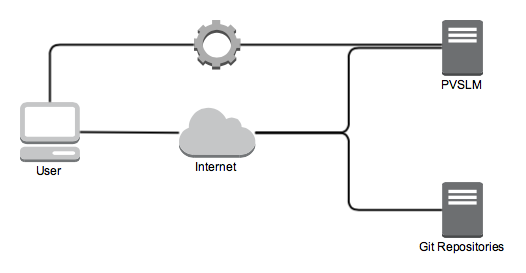
\includegraphics[scale=0.5]{archi}
  \caption{PVS Library Manager architecture}
  \label{fig:archi}
\end{figure}

